\section{Potential Fields}
	Potential fields can be used to move a computer AI through a dynamically updated environment. 
	If one would program an AI which should move from one point to another, one would most likely use a normal shortest path algorithms. 
	The problem is that if there are a lot of dynamic influences effect the route, this calculation becomes very complex. It could be 
	enemies that should be avoided or other dynamic influences. \\
	
	This is why potential fields are good for such a problem. They work by generating either attractive or repulsive fields of vectors $v=(m\times d )$. 
	Where $m$ is the magnitude and $d$ is the direction. 
	If we create an attractive potential field the point will be surrounded by vectors pointing toward this point, 
	as seen in figure \ref{fig:seekbehavior}. 
	The bot will be attracted towards this point. The magnitude determines how attractive the field will be. The direction shows in which way the bot is will move. This is called a Attractive behaviour 
		
	\begin{figure}[H]
		\begin{center}
			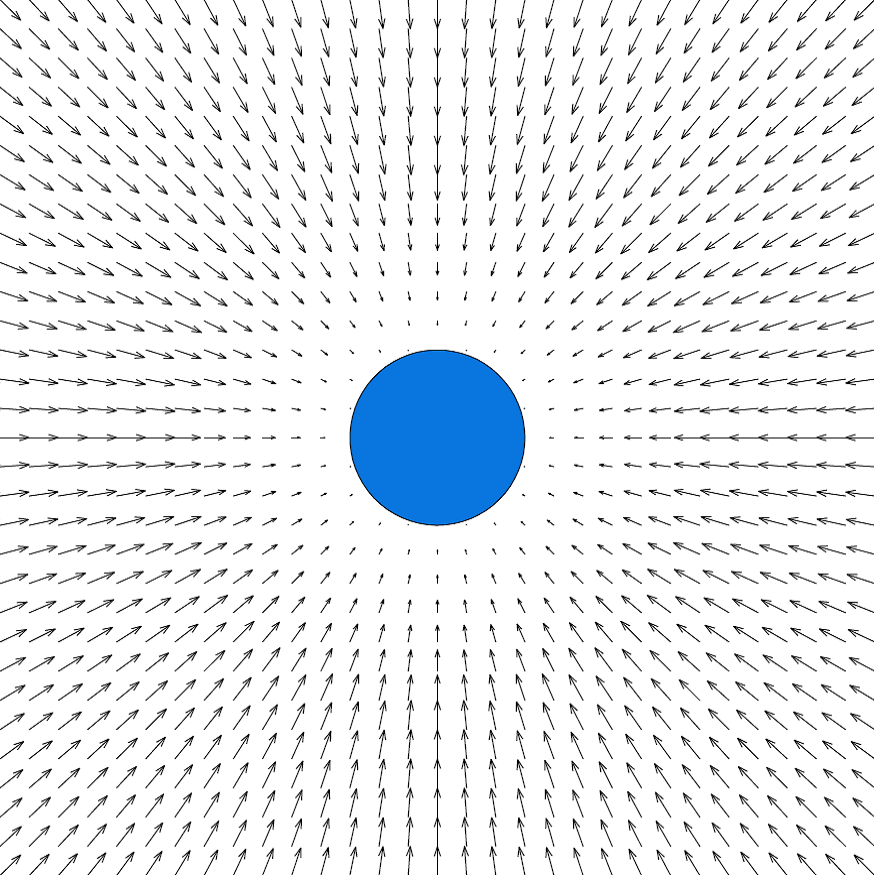
\includegraphics[scale=0.3]{Figures/Potentialfields/seek.png}
			\caption{Attractive behavior\cite{pft}}\label{fig:seekbehavior}
		\end{center}
	\end{figure}
	
	Likewise if we assume there is only a single obstacles in the area (a unit we do not want to attack) it would generate a repulsive field around it, 
	see figure \ref{fig:avoidbehavior}. This is called a repulsive behaviour because it causes our own units to try and avoid it.

		
	\begin{figure}[H]
		\begin{center}
			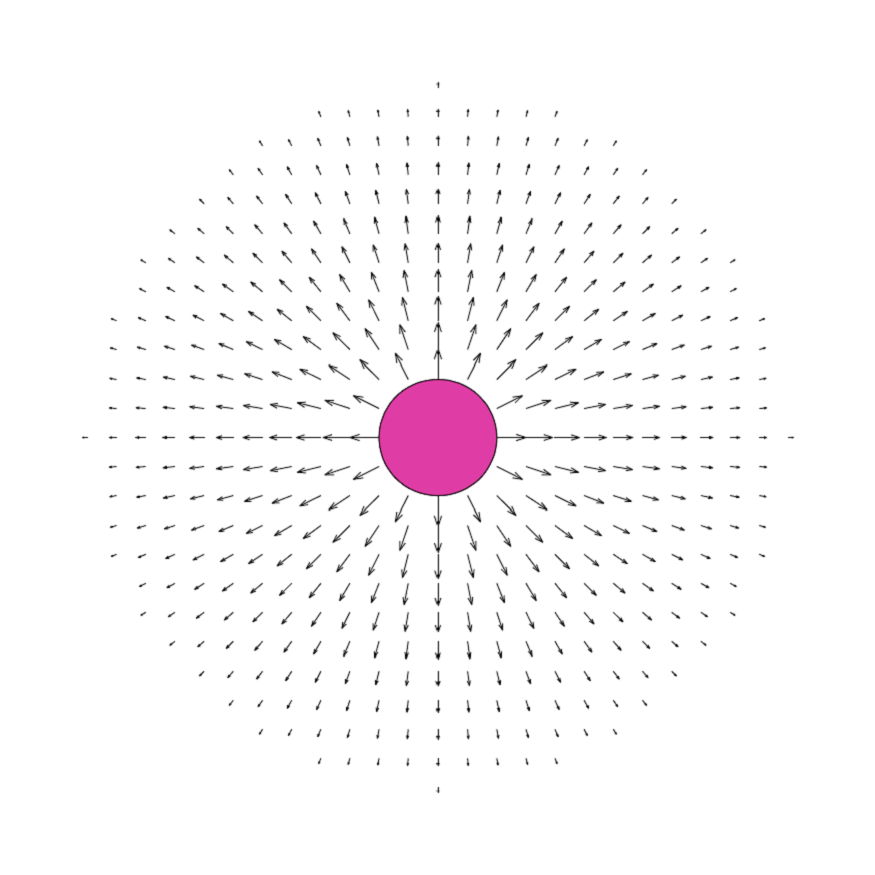
\includegraphics[scale=0.3]{Figures/Potentialfields/avoid.png}
			\caption{Repulsive behavior\cite{pft}}\label{fig:avoidbehavior}
		\end{center}
	\end{figure}
		
	These two kinds of behaviours can be combined to make a map that can tell our unit 
	how to move around enemy units and reach a specific target as seen in figure \ref{fig:combinedbehavior}.
			
	\begin{figure}[H]
		\begin{center}
			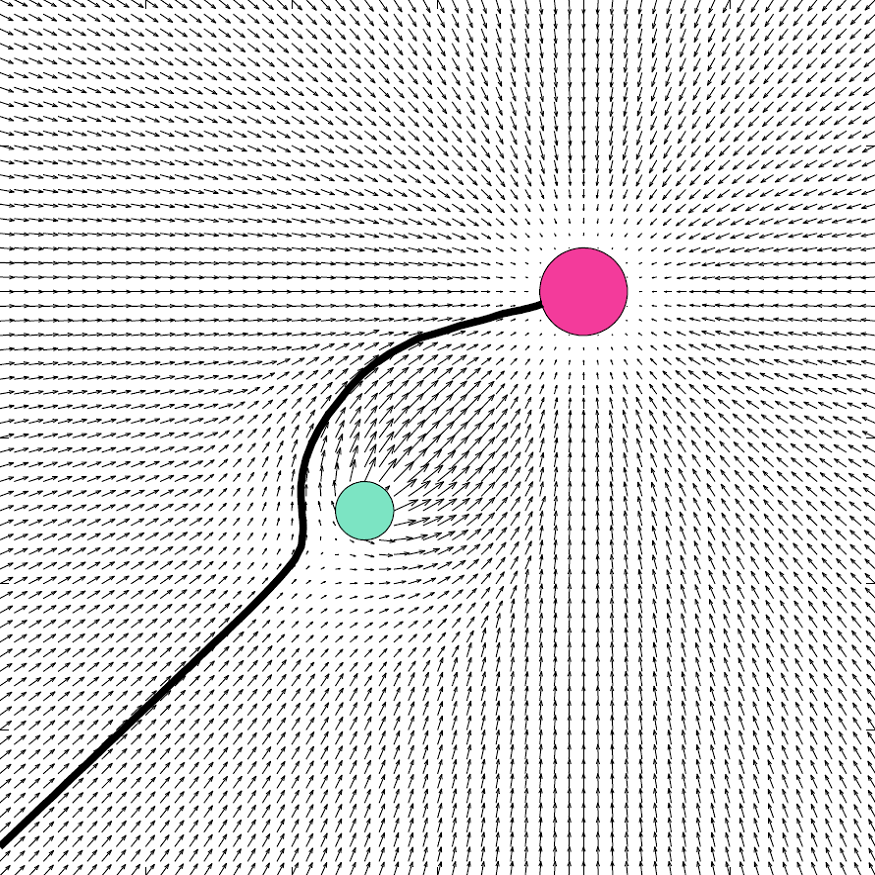
\includegraphics[scale=0.3]{Figures/Potentialfields/combined.png}
			\caption{Combined behavior\cite{pft}}\label{fig:combinedbehavior}
			\end{center}
	\end{figure}
		
	
	\subsection{Designing our Potential Field Functions}		
		The potential fields in our bot will reduce the vectors into constant values that represent their importance or magnitude. We arrange the vector to fit linear values that indicate how attractive or repulsive a field is. 
		This number is calculated by functions, which is either attractive or repulsive and is related to the obstacles in the game world. 
		
		The reason we can use numbers instead of vectors is because we only care about the potential on the tiles 
		\footnote{A tile represents an 8px$\times8px$ square. 
		This is the smallest area a units can stand on or move to.} 
		immediately surrounding a unit, so the direction is given by just taking the highest number. As seen in figure \ref{fig:vectorsAsNumbers}.
		\insertmarginfigure{height=1.5in}{Potentialfields/vectors.png}
		{Vector direction given by numbers}{fig:vectorsAsNumbers}{-3in}
		\\
		
		\subsubsection{Potential Field Basic Structure}
		Our functions will be described with the following math\cite{ptlp}: \\
		
		Variables:\\
		$f =$ force\\
		$s =$ size of the potential field\\
		$c =$ constant\\
		$d =$ distance\\
		
		\begin{displaymath}
			%\begin{math}
			Attractive = \begin{cases}
					f * c & \text{if $d > s$}\\
					0 & \text{else}
				\end{cases}		
			%\end{math}
		\end{displaymath}
			
		\begin{displaymath}
			%\begin{math}
			Repulsive = \begin{cases}
					- f * c & \text{if $d > s$}\\
					0 & \text{else}
				\end{cases}		
			%\end{math}
		\end{displaymath}
		
		
